\documentclass[twoside]{book}

% Packages required by doxygen
\usepackage{fixltx2e}
\usepackage{calc}
\usepackage{doxygen}
\usepackage[export]{adjustbox} % also loads graphicx
\usepackage{graphicx}
\usepackage[utf8]{inputenc}
\usepackage{makeidx}
\usepackage{multicol}
\usepackage{multirow}
\PassOptionsToPackage{warn}{textcomp}
\usepackage{textcomp}
\usepackage[nointegrals]{wasysym}
\usepackage[table]{xcolor}

% Font selection
\usepackage[T1]{fontenc}
\usepackage[scaled=.90]{helvet}
\usepackage{courier}
\usepackage{amssymb}
\usepackage{sectsty}
\renewcommand{\familydefault}{\sfdefault}
\allsectionsfont{%
  \fontseries{bc}\selectfont%
  \color{darkgray}%
}
\renewcommand{\DoxyLabelFont}{%
  \fontseries{bc}\selectfont%
  \color{darkgray}%
}
\newcommand{\+}{\discretionary{\mbox{\scriptsize$\hookleftarrow$}}{}{}}

% Page & text layout
\usepackage{geometry}
\geometry{%
  a4paper,%
  top=2.5cm,%
  bottom=2.5cm,%
  left=2.5cm,%
  right=2.5cm%
}
\tolerance=750
\hfuzz=15pt
\hbadness=750
\setlength{\emergencystretch}{15pt}
\setlength{\parindent}{0cm}
\setlength{\parskip}{0.2cm}
\makeatletter
\renewcommand{\paragraph}{%
  \@startsection{paragraph}{4}{0ex}{-1.0ex}{1.0ex}{%
    \normalfont\normalsize\bfseries\SS@parafont%
  }%
}
\renewcommand{\subparagraph}{%
  \@startsection{subparagraph}{5}{0ex}{-1.0ex}{1.0ex}{%
    \normalfont\normalsize\bfseries\SS@subparafont%
  }%
}
\makeatother

% Headers & footers
\usepackage{fancyhdr}
\pagestyle{fancyplain}
\fancyhead[LE]{\fancyplain{}{\bfseries\thepage}}
\fancyhead[CE]{\fancyplain{}{}}
\fancyhead[RE]{\fancyplain{}{\bfseries\leftmark}}
\fancyhead[LO]{\fancyplain{}{\bfseries\rightmark}}
\fancyhead[CO]{\fancyplain{}{}}
\fancyhead[RO]{\fancyplain{}{\bfseries\thepage}}
\fancyfoot[LE]{\fancyplain{}{}}
\fancyfoot[CE]{\fancyplain{}{}}
\fancyfoot[RE]{\fancyplain{}{\bfseries\scriptsize Generated on Sun Jan 17 2016 10\+:35\+:00 for project\+\_\+template by Doxygen }}
\fancyfoot[LO]{\fancyplain{}{\bfseries\scriptsize Generated on Sun Jan 17 2016 10\+:35\+:00 for project\+\_\+template by Doxygen }}
\fancyfoot[CO]{\fancyplain{}{}}
\fancyfoot[RO]{\fancyplain{}{}}
\renewcommand{\footrulewidth}{0.4pt}
\renewcommand{\chaptermark}[1]{%
  \markboth{#1}{}%
}
\renewcommand{\sectionmark}[1]{%
  \markright{\thesection\ #1}%
}

% Indices & bibliography
\usepackage{natbib}
\usepackage[titles]{tocloft}
\setcounter{tocdepth}{3}
\setcounter{secnumdepth}{5}
\makeindex

% Hyperlinks (required, but should be loaded last)
\usepackage{ifpdf}
\ifpdf
  \usepackage[pdftex,pagebackref=true]{hyperref}
\else
  \usepackage[ps2pdf,pagebackref=true]{hyperref}
\fi
\hypersetup{%
  colorlinks=true,%
  linkcolor=blue,%
  citecolor=blue,%
  unicode%
}

% Custom commands
\newcommand{\clearemptydoublepage}{%
  \newpage{\pagestyle{empty}\cleardoublepage}%
}


%===== C O N T E N T S =====

\begin{document}

% Titlepage & ToC
\hypersetup{pageanchor=false,
             bookmarks=true,
             bookmarksnumbered=true,
             pdfencoding=unicode
            }
\pagenumbering{roman}
\begin{titlepage}
\vspace*{7cm}
\begin{center}%
{\Large project\+\_\+template \\[1ex]\large x.\+x.\+x }\\
\vspace*{1cm}
{\large Generated by Doxygen 1.8.10}\\
\vspace*{0.5cm}
{\small Sun Jan 17 2016 10:35:00}\\
\end{center}
\end{titlepage}
\clearemptydoublepage
\tableofcontents
\clearemptydoublepage
\pagenumbering{arabic}
\hypersetup{pageanchor=true}

%--- Begin generated contents ---
\chapter{provide title for project}
\label{index}\hypertarget{index}{}{\itshape {\bfseries Introduction} {\bfseries to} {\bfseries template}  } \begin{DoxyNote}{Note}
You may use this template to produce your source code, which is documented and coded as per the stipulated standards. This template is produced using Eclipse I\+D\+E and Doxygen document generation tool. You may refer to Documentation and Coding Standards -\/ Guidelines for more details; or you may visit respective official web-\/site. ~\newline
\begin{TabularC}{2}
\hline
\rowcolor{lightgray}{\bf Description }&{\bf Web-\/link/\+Document  }\\\cline{1-2}
Documentation and Coding Standards -\/ Guidelines &documentation\+\_\+and\+\_\+coding\+\_\+standard\+\_\+guidelines.\+pdf \\\cline{1-2}
Doxygen Command Reference &doxygen\+\_\+command\+\_\+reference.\+pdf \\\cline{1-2}
Doxygen Document Generation &\href{http://www.stack.nl/~dimitri/doxygen}{\tt Doxygen} \\\cline{1-2}
G\+N\+U Coding Standards &\href{http://www.gnu.org/prep/standards/standards.html}{\tt G\+N\+U Coding Standards} \\\cline{1-2}
\end{TabularC}

\end{DoxyNote}
\begin{DoxyAttention}{Attention}
Remember to remove and/or replace each section/topic of source file and respective documentation with relevant and applicable information applicable to your project. 
\end{DoxyAttention}
\begin{DoxyWarning}{Warning}
It is recommended and required to read through and understand the concepts from respective guide before attempting to use this template.
\end{DoxyWarning}




\begin{DoxyAuthor}{Author}
provide author details 
\end{DoxyAuthor}
\begin{DoxyDate}{Date}
provide date 
\end{DoxyDate}
\begin{DoxyCopyright}{Copyright}
provide copyright information 
\end{DoxyCopyright}
\begin{DoxyParagraph}{You may provide an overview of the project. Details can be organized in multiple sections and subsection.}
Replace below the section/subsection names and corresponding description/details according to need. 
\end{DoxyParagraph}
\hypertarget{index_section_name_1}{}\section{Section 1 provide section name and description}\label{index_section_name_1}
\begin{DoxyParagraph}{Put your Paragraph describing section}
~\newline

\end{DoxyParagraph}
\hypertarget{index_subsection_name_1_1}{}\subsection{Subsection 1.\+1 provide subsection name and description}\label{index_subsection_name_1_1}
\begin{DoxyParagraph}{(paragraph -\/ 01)}

\end{DoxyParagraph}
\begin{DoxyParagraph}{(paragraph -\/ 02)}
~\newline
~\newline

\end{DoxyParagraph}
\hypertarget{index_section_name_2}{}\section{Section 2 provide section name and description}\label{index_section_name_2}
\begin{DoxyParagraph}{Put your Paragraph describing section}

\end{DoxyParagraph}
\hypertarget{index_subsection_name_2_1}{}\subsection{Subsection 2.\+1 provide subsection name and description}\label{index_subsection_name_2_1}
\begin{DoxyParagraph}{(paragraph -\/ 01)}

\end{DoxyParagraph}
\begin{DoxyParagraph}{(paragraph -\/ 02)}

\end{DoxyParagraph}
\begin{DoxyParagraph}{}

\end{DoxyParagraph}


 
\chapter{Release Notes\+:}
\label{product_release_main_page}
\hypertarget{product_release_main_page}{}
Foreword\+: provide brief description

This product release document is divided in the following sections\+:
\begin{DoxyItemize}
\item \hyperlink{introduction}{Introduction}
\item \hyperlink{requirements}{Requirements}
\item \hyperlink{hardware_design}{Hardware Design}
\item \hyperlink{software_design}{Software Design}
\end{DoxyItemize}

For details on source code and related documentation visit respective section. \hypertarget{introduction}{}\section{Introduction}\label{introduction}
Provide introduction, and abstract view of product function, and list of hardware

List of hardware\+:
\begin{DoxyItemize}
\item \hyperlink{hardware_design_hw_section_01}{Section 01}.
\item \hyperlink{hardware_design_hw_section_02}{Section 02}.
\end{DoxyItemize}

Go back to \hyperlink{product_release_main_page}{Release Note\+:Main Menu}. \hypertarget{requirements}{}\section{Requirements}\label{requirements}
Provide details of functional requirements for the sprint.

Go back to \hyperlink{product_release_main_page}{Release Note\+:Main Menu}. \hypertarget{hardware_design}{}\section{Hardwre Design}\label{hardware_design}
provide brief details for this section.\hypertarget{hardware_design_hw_section_01}{}\subsection{Section 01}\label{hardware_design_hw_section_01}
To load an image set the parameter I\+M\+A\+G\+E\+\_\+\+P\+A\+T\+H to appropriate folder in doxyfile for the project\hypertarget{hardware_design_hw_subsection_01}{}\subsubsection{Subsction 01}\label{hardware_design_hw_subsection_01}
provide details
\begin{DoxyItemize}
\item \hyperlink{hardware_design_hw_section_02}{Section 02} Section 02
\item \hyperlink{hardware_design_hw_section_03}{Section 03} Section 03
\end{DoxyItemize}\hypertarget{hardware_design_hw_subsection_02}{}\subsubsection{hw\+\_\+subsection\+\_\+02}\label{hardware_design_hw_subsection_02}
Table \begin{TabularC}{3}
\hline
\rowcolor{lightgray}{\bf Column 1 }&{\bf Column 2 }&{\bf Details  }\\\cline{1-3}
Details &Details &Details \\\cline{1-3}
Details &Details &Details \\\cline{1-3}
Details &Details &Details \\\cline{1-3}
\end{TabularC}


Go to \hyperlink{hardware_design}{Top} / \hyperlink{product_release_main_page}{Release Note\+:Main Menu}.

~\newline
~\newline
\hypertarget{hardware_design_hw_section_02}{}\subsection{Section 02}\label{hardware_design_hw_section_02}
To load an image set the parameter I\+M\+A\+G\+E\+\_\+\+P\+A\+T\+H to appropriate folder in doxyfile for the project\hypertarget{hardware_design_hw_subsection_04}{}\subsubsection{Subsection 04}\label{hardware_design_hw_subsection_04}
~\newline
Go to \hyperlink{hardware_design}{Top} / \hyperlink{product_release_main_page}{Release Note\+:Main Menu}.

~\newline
 ~\newline
\hypertarget{hardware_design_hw_section_03}{}\subsection{Section 03}\label{hardware_design_hw_section_03}
\hypertarget{hardware_design_hw_subsection_05}{}\subsubsection{Subsection 05}\label{hardware_design_hw_subsection_05}
Go to \hyperlink{hardware_design}{Top} / \hyperlink{product_release_main_page}{Release Note\+:Main Menu}. \hypertarget{software_design}{}\section{Software Design}\label{software_design}
provide brief details for this section.\hypertarget{software_design_sw_section_01}{}\subsection{Section 01}\label{software_design_sw_section_01}
To load an image set the parameter I\+M\+A\+G\+E\+\_\+\+P\+A\+T\+H to appropriate folder in doxyfile for the project\hypertarget{software_design_sw_subsection_01}{}\subsubsection{Subsction 01}\label{software_design_sw_subsection_01}
provide details
\begin{DoxyItemize}
\item \hyperlink{software_design_sw_section_02}{Section 02} Section 02
\item \hyperlink{software_design_sw_section_03}{Section 03} Section 03
\end{DoxyItemize}\hypertarget{software_design_sw_subsection_02}{}\subsubsection{sw\+\_\+subsection\+\_\+02}\label{software_design_sw_subsection_02}
Table \begin{TabularC}{3}
\hline
\rowcolor{lightgray}{\bf Column 1 }&{\bf Column 2 }&{\bf Details  }\\\cline{1-3}
Details &Details &Details \\\cline{1-3}
Details &Details &Details \\\cline{1-3}
Details &Details &Details \\\cline{1-3}
\end{TabularC}


Go to \hyperlink{software_design}{Top} / \hyperlink{product_release_main_page}{Release Note\+:Main Menu}.

~\newline
~\newline
\hypertarget{software_design_sw_section_02}{}\subsection{Section 02}\label{software_design_sw_section_02}
To load an image set the parameter I\+M\+A\+G\+E\+\_\+\+P\+A\+T\+H to appropriate folder in doxyfile for the project\hypertarget{software_design_sw_subsection_04}{}\subsubsection{Subsection 04}\label{software_design_sw_subsection_04}
~\newline
Go to \hyperlink{software_design}{Top} / \hyperlink{product_release_main_page}{Release Note\+:Main Menu}.

~\newline
 ~\newline
\hypertarget{software_design_sw_section_03}{}\subsection{Section 03}\label{software_design_sw_section_03}
\hypertarget{software_design_sw_subsection_05}{}\subsubsection{Subsection 05}\label{software_design_sw_subsection_05}
Go to \hyperlink{software_design}{Top} / \hyperlink{product_release_main_page}{Release Note\+:Main Menu}. 
\chapter{File Index}
\section{File List}
Here is a list of all documented files with brief descriptions\+:\begin{DoxyCompactList}
\item\contentsline{section}{{\bf usart\+Serial.\+c} \\*Module for asynchronous communication with the Atmega2560 U\+S\+A\+R\+T\textquotesingle{}s }{\pageref{usart_serial_8c}}{}
\end{DoxyCompactList}

\chapter{File Documentation}
\hypertarget{template_8h}{}\section{include/template.h File Reference}
\label{template_8h}\index{include/template.\+h@{include/template.\+h}}


Provide short summary on function and the contents of file.  


{\ttfamily \#include $<$stdlib.\+h$>$}\\*
Include dependency graph for template.\+h\+:\nopagebreak
\begin{figure}[H]
\begin{center}
\leavevmode
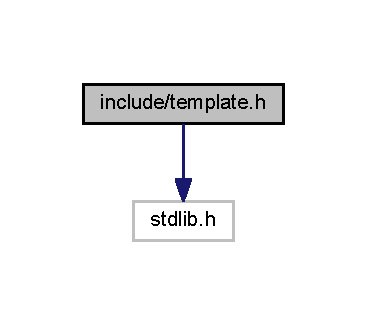
\includegraphics[width=176pt]{template_8h__incl}
\end{center}
\end{figure}
This graph shows which files directly or indirectly include this file\+:\nopagebreak
\begin{figure}[H]
\begin{center}
\leavevmode
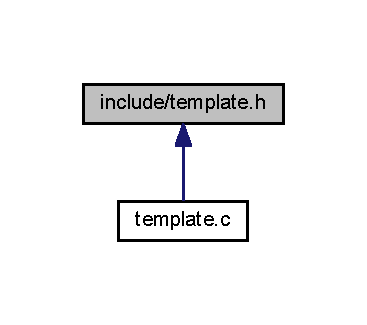
\includegraphics[width=176pt]{template_8h__dep__incl}
\end{center}
\end{figure}
\subsection*{Macros}
\begin{DoxyCompactItemize}
\item 
\#define \hyperlink{template_8h_a7138ed1511a8cbd3c982ce20071a83b7}{M\+A\+C\+R\+O\+\_\+\+H\+F}~000
\end{DoxyCompactItemize}
\subsection*{Functions}
\begin{DoxyCompactItemize}
\item 
void \hyperlink{template_8h_a8210bf00ef427ddd7cb7ac758778356c}{entry\+\_\+point\+\_\+function\+\_\+one} (int parameter\+\_\+one, float parameter\+\_\+two, char $\ast$parameter\+\_\+three, float parameter\+\_\+four, int parameter\+\_\+five)
\begin{DoxyCompactList}\small\item\em Provide short description on functionality of function. \end{DoxyCompactList}\item 
void \hyperlink{template_8h_a3bb155d761781f687f13cea299618968}{entry\+\_\+point\+\_\+function\+\_\+two} (int parameter\+\_\+one, float parameter\+\_\+two, char $\ast$parameter\+\_\+three)
\begin{DoxyCompactList}\small\item\em Provide short description on functionality of function. \end{DoxyCompactList}\end{DoxyCompactItemize}
\subsection*{Variables}
\begin{DoxyCompactItemize}
\item 
int \hyperlink{template_8h_a35eef0621f3687d2b6fe9712fbd68b55}{global\+\_\+variable\+\_\+hf}
\end{DoxyCompactItemize}


\subsection{Detailed Description}
Provide short summary on function and the contents of file. 

\begin{DoxyAuthor}{Author}
provide author details 
\end{DoxyAuthor}
\begin{DoxyDate}{Date}
provide date
\end{DoxyDate}
Provide detailed description 

\subsection{Macro Definition Documentation}
\hypertarget{template_8h_a7138ed1511a8cbd3c982ce20071a83b7}{}\index{template.\+h@{template.\+h}!M\+A\+C\+R\+O\+\_\+\+H\+F@{M\+A\+C\+R\+O\+\_\+\+H\+F}}
\index{M\+A\+C\+R\+O\+\_\+\+H\+F@{M\+A\+C\+R\+O\+\_\+\+H\+F}!template.\+h@{template.\+h}}
\subsubsection[{M\+A\+C\+R\+O\+\_\+\+H\+F}]{\setlength{\rightskip}{0pt plus 5cm}\#define M\+A\+C\+R\+O\+\_\+\+H\+F~000}\label{template_8h_a7138ed1511a8cbd3c982ce20071a83b7}
Provide description for documentation purpose 

Definition at line 68 of file template.\+h.



\subsection{Function Documentation}
\hypertarget{template_8h_a8210bf00ef427ddd7cb7ac758778356c}{}\index{template.\+h@{template.\+h}!entry\+\_\+point\+\_\+function\+\_\+one@{entry\+\_\+point\+\_\+function\+\_\+one}}
\index{entry\+\_\+point\+\_\+function\+\_\+one@{entry\+\_\+point\+\_\+function\+\_\+one}!template.\+h@{template.\+h}}
\subsubsection[{entry\+\_\+point\+\_\+function\+\_\+one(int parameter\+\_\+one, float parameter\+\_\+two, char $\ast$parameter\+\_\+three, float parameter\+\_\+four, int parameter\+\_\+five)}]{\setlength{\rightskip}{0pt plus 5cm}void entry\+\_\+point\+\_\+function\+\_\+one (
\begin{DoxyParamCaption}
\item[{int}]{parameter\+\_\+one, }
\item[{float}]{parameter\+\_\+two, }
\item[{char $\ast$}]{parameter\+\_\+three, }
\item[{float}]{parameter\+\_\+four, }
\item[{int}]{parameter\+\_\+five}
\end{DoxyParamCaption}
)}\label{template_8h_a8210bf00ef427ddd7cb7ac758778356c}


Provide short description on functionality of function. 

Provide detailed description of function, including calling mechanism and return value.
\begin{DoxyItemize}
\item Functions
\begin{DoxyEnumerate}
\item Function ...1
\item Function ...2
\item Function ...3
\end{DoxyEnumerate}
\end{DoxyItemize}


\begin{DoxyParams}{Parameters}
{\em parameter\+\_\+one} & Provide description \\
\hline
{\em parameter\+\_\+two} & Provide description \\
\hline
{\em parameter\+\_\+three} & Provide description \\
\hline
{\em parameter\+\_\+four} & Provide description \\
\hline
{\em parameter\+\_\+five} & Provide description \\
\hline
\end{DoxyParams}
\begin{DoxyReturn}{Returns}

\end{DoxyReturn}


Definition at line 156 of file template.\+c.

\hypertarget{template_8h_a3bb155d761781f687f13cea299618968}{}\index{template.\+h@{template.\+h}!entry\+\_\+point\+\_\+function\+\_\+two@{entry\+\_\+point\+\_\+function\+\_\+two}}
\index{entry\+\_\+point\+\_\+function\+\_\+two@{entry\+\_\+point\+\_\+function\+\_\+two}!template.\+h@{template.\+h}}
\subsubsection[{entry\+\_\+point\+\_\+function\+\_\+two(int parameter\+\_\+one, float parameter\+\_\+two, char $\ast$parameter\+\_\+three)}]{\setlength{\rightskip}{0pt plus 5cm}void entry\+\_\+point\+\_\+function\+\_\+two (
\begin{DoxyParamCaption}
\item[{int}]{parameter\+\_\+one, }
\item[{float}]{parameter\+\_\+two, }
\item[{char $\ast$}]{parameter\+\_\+three}
\end{DoxyParamCaption}
)}\label{template_8h_a3bb155d761781f687f13cea299618968}


Provide short description on functionality of function. 

Provide detailed description of function, including calling mechanism and return value.


\begin{DoxyParams}{Parameters}
{\em parameter\+\_\+one} & Provide description \\
\hline
{\em parameter\+\_\+two} & Provide description \\
\hline
{\em parameter\+\_\+three} & Provide description \\
\hline
\end{DoxyParams}
\begin{DoxyReturn}{Returns}

\end{DoxyReturn}


Definition at line 172 of file template.\+c.



\subsection{Variable Documentation}
\hypertarget{template_8h_a35eef0621f3687d2b6fe9712fbd68b55}{}\index{template.\+h@{template.\+h}!global\+\_\+variable\+\_\+hf@{global\+\_\+variable\+\_\+hf}}
\index{global\+\_\+variable\+\_\+hf@{global\+\_\+variable\+\_\+hf}!template.\+h@{template.\+h}}
\subsubsection[{global\+\_\+variable\+\_\+hf}]{\setlength{\rightskip}{0pt plus 5cm}int global\+\_\+variable\+\_\+hf}\label{template_8h_a35eef0621f3687d2b6fe9712fbd68b55}
Provide description for documentation purpose 

Definition at line 85 of file template.\+h.


\hypertarget{mainpage_8dox}{}\section{mainpage.\+dox File Reference}
\label{mainpage_8dox}\index{mainpage.\+dox@{mainpage.\+dox}}

\hypertarget{product__release__document_8dox}{}\section{product\+\_\+release\+\_\+document.\+dox File Reference}
\label{product__release__document_8dox}\index{product\+\_\+release\+\_\+document.\+dox@{product\+\_\+release\+\_\+document.\+dox}}

\hypertarget{template_8c}{}\section{template.\+c File Reference}
\label{template_8c}\index{template.\+c@{template.\+c}}


Provide short summary on function and the contents of file.  


{\ttfamily \#include \char`\"{}template.\+h\char`\"{}}\\*
{\ttfamily \#include $<$stdio.\+h$>$}\\*
{\ttfamily \#include \char`\"{}avr/io.\+h\char`\"{}}\\*
{\ttfamily \#include \char`\"{}avr/interrupt.\+h\char`\"{}}\\*
Include dependency graph for template.\+c\+:\nopagebreak
\begin{figure}[H]
\begin{center}
\leavevmode
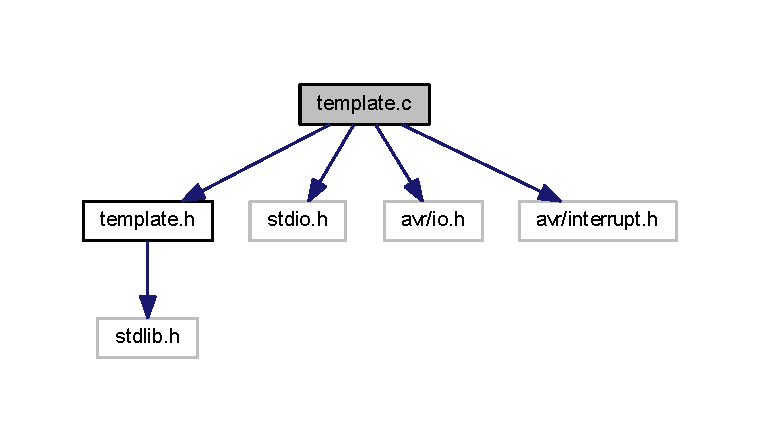
\includegraphics[width=350pt]{template_8c__incl}
\end{center}
\end{figure}
\subsection*{Macros}
\begin{DoxyCompactItemize}
\item 
\#define \hyperlink{template_8c_aa292137032b645eef0bb9f5008b737b9}{M\+A\+C\+R\+O\+\_\+\+S\+F}~999
\end{DoxyCompactItemize}
\subsection*{Functions}
\begin{DoxyCompactItemize}
\item 
int \hyperlink{template_8c_a840291bc02cba5474a4cb46a9b9566fe}{main} (void)
\begin{DoxyCompactList}\small\item\em Main entry point for the program. Provide short description. \end{DoxyCompactList}\item 
void \hyperlink{template_8c_a8210bf00ef427ddd7cb7ac758778356c}{entry\+\_\+point\+\_\+function\+\_\+one} (int parameter\+\_\+one, float parameter\+\_\+two, char $\ast$parameter\+\_\+three, float parameter\+\_\+four, int parameter\+\_\+five)
\begin{DoxyCompactList}\small\item\em Provide short description on functionality of function. \end{DoxyCompactList}\item 
void \hyperlink{template_8c_a3bb155d761781f687f13cea299618968}{entry\+\_\+point\+\_\+function\+\_\+two} (int parameter\+\_\+one, float parameter\+\_\+two, char $\ast$parameter\+\_\+three)
\begin{DoxyCompactList}\small\item\em Provide short description on functionality of function. \end{DoxyCompactList}\item 
float \hyperlink{template_8c_ae15c1828ca7bb40709c3b4b1224c02cc}{local\+\_\+function\+\_\+one} (int parameter\+\_\+one, float parameter\+\_\+two, char $\ast$parameter\+\_\+three)
\begin{DoxyCompactList}\small\item\em Provide short description on functionality of function. \end{DoxyCompactList}\item 
float \hyperlink{template_8c_a6493901a6ddd614d6f9b0d3d72d0d414}{local\+\_\+function\+\_\+two} (int parameter\+\_\+one, float parameter\+\_\+two, char $\ast$parameter\+\_\+three, float parameter\+\_\+four, int parameter\+\_\+five)
\begin{DoxyCompactList}\small\item\em Provide short description on functionality of function. \end{DoxyCompactList}\item 
\hyperlink{template_8c_a1b97fa4a9ffcf4b70a6403ba26fd3a5c}{I\+S\+R} (I\+N\+T4\+\_\+vect, I\+S\+R\+\_\+\+B\+L\+O\+C\+K)
\begin{DoxyCompactList}\small\item\em Provide short description on interrupt service routine. \end{DoxyCompactList}\item 
\hyperlink{template_8c_a451a644f2b139393fc1fe1cf7373cb93}{I\+S\+R} (U\+S\+A\+R\+T0\+\_\+\+R\+X\+\_\+vect, I\+S\+R\+\_\+\+B\+L\+O\+C\+K)
\begin{DoxyCompactList}\small\item\em Provide short description on interrupt service routine. \end{DoxyCompactList}\end{DoxyCompactItemize}
\subsection*{Variables}
\begin{DoxyCompactItemize}
\item 
int \hyperlink{template_8c_a395dbc90e8c7a0ac05b0cf8c6438b7e5}{global\+\_\+variable\+\_\+sf}
\end{DoxyCompactItemize}


\subsection{Detailed Description}
Provide short summary on function and the contents of file. 

\begin{DoxyAuthor}{Author}
provide author details 
\end{DoxyAuthor}
\begin{DoxyDate}{Date}
provide date
\end{DoxyDate}
Provide detailed description 

\subsection{Macro Definition Documentation}
\hypertarget{template_8c_aa292137032b645eef0bb9f5008b737b9}{}\index{template.\+c@{template.\+c}!M\+A\+C\+R\+O\+\_\+\+S\+F@{M\+A\+C\+R\+O\+\_\+\+S\+F}}
\index{M\+A\+C\+R\+O\+\_\+\+S\+F@{M\+A\+C\+R\+O\+\_\+\+S\+F}!template.\+c@{template.\+c}}
\subsubsection[{M\+A\+C\+R\+O\+\_\+\+S\+F}]{\setlength{\rightskip}{0pt plus 5cm}\#define M\+A\+C\+R\+O\+\_\+\+S\+F~999}\label{template_8c_aa292137032b645eef0bb9f5008b737b9}
Provide description for documentation purpose 

Definition at line 60 of file template.\+c.



\subsection{Function Documentation}
\hypertarget{template_8c_a8210bf00ef427ddd7cb7ac758778356c}{}\index{template.\+c@{template.\+c}!entry\+\_\+point\+\_\+function\+\_\+one@{entry\+\_\+point\+\_\+function\+\_\+one}}
\index{entry\+\_\+point\+\_\+function\+\_\+one@{entry\+\_\+point\+\_\+function\+\_\+one}!template.\+c@{template.\+c}}
\subsubsection[{entry\+\_\+point\+\_\+function\+\_\+one(int parameter\+\_\+one, float parameter\+\_\+two, char $\ast$parameter\+\_\+three, float parameter\+\_\+four, int parameter\+\_\+five)}]{\setlength{\rightskip}{0pt plus 5cm}void entry\+\_\+point\+\_\+function\+\_\+one (
\begin{DoxyParamCaption}
\item[{int}]{parameter\+\_\+one, }
\item[{float}]{parameter\+\_\+two, }
\item[{char $\ast$}]{parameter\+\_\+three, }
\item[{float}]{parameter\+\_\+four, }
\item[{int}]{parameter\+\_\+five}
\end{DoxyParamCaption}
)}\label{template_8c_a8210bf00ef427ddd7cb7ac758778356c}


Provide short description on functionality of function. 

Provide detailed description of function, including calling mechanism and return value.
\begin{DoxyItemize}
\item Functions
\begin{DoxyEnumerate}
\item Function ...1
\item Function ...2
\item Function ...3
\end{DoxyEnumerate}
\end{DoxyItemize}


\begin{DoxyParams}{Parameters}
{\em parameter\+\_\+one} & Provide description \\
\hline
{\em parameter\+\_\+two} & Provide description \\
\hline
{\em parameter\+\_\+three} & Provide description \\
\hline
{\em parameter\+\_\+four} & Provide description \\
\hline
{\em parameter\+\_\+five} & Provide description \\
\hline
\end{DoxyParams}
\begin{DoxyReturn}{Returns}

\end{DoxyReturn}


Definition at line 156 of file template.\+c.

\hypertarget{template_8c_a3bb155d761781f687f13cea299618968}{}\index{template.\+c@{template.\+c}!entry\+\_\+point\+\_\+function\+\_\+two@{entry\+\_\+point\+\_\+function\+\_\+two}}
\index{entry\+\_\+point\+\_\+function\+\_\+two@{entry\+\_\+point\+\_\+function\+\_\+two}!template.\+c@{template.\+c}}
\subsubsection[{entry\+\_\+point\+\_\+function\+\_\+two(int parameter\+\_\+one, float parameter\+\_\+two, char $\ast$parameter\+\_\+three)}]{\setlength{\rightskip}{0pt plus 5cm}void entry\+\_\+point\+\_\+function\+\_\+two (
\begin{DoxyParamCaption}
\item[{int}]{parameter\+\_\+one, }
\item[{float}]{parameter\+\_\+two, }
\item[{char $\ast$}]{parameter\+\_\+three}
\end{DoxyParamCaption}
)}\label{template_8c_a3bb155d761781f687f13cea299618968}


Provide short description on functionality of function. 

Provide detailed description of function, including calling mechanism and return value.


\begin{DoxyParams}{Parameters}
{\em parameter\+\_\+one} & Provide description \\
\hline
{\em parameter\+\_\+two} & Provide description \\
\hline
{\em parameter\+\_\+three} & Provide description \\
\hline
\end{DoxyParams}
\begin{DoxyReturn}{Returns}

\end{DoxyReturn}


Definition at line 172 of file template.\+c.

\hypertarget{template_8c_a1b97fa4a9ffcf4b70a6403ba26fd3a5c}{}\index{template.\+c@{template.\+c}!I\+S\+R@{I\+S\+R}}
\index{I\+S\+R@{I\+S\+R}!template.\+c@{template.\+c}}
\subsubsection[{I\+S\+R(\+I\+N\+T4\+\_\+vect, I\+S\+R\+\_\+\+B\+L\+O\+C\+K)}]{\setlength{\rightskip}{0pt plus 5cm}I\+S\+R (
\begin{DoxyParamCaption}
\item[{I\+N\+T4\+\_\+vect}]{, }
\item[{I\+S\+R\+\_\+\+B\+L\+O\+C\+K}]{}
\end{DoxyParamCaption}
)}\label{template_8c_a1b97fa4a9ffcf4b70a6403ba26fd3a5c}


Provide short description on interrupt service routine. 

Provide detailed description of interrupt service routine 

Definition at line 232 of file template.\+c.

\hypertarget{template_8c_a451a644f2b139393fc1fe1cf7373cb93}{}\index{template.\+c@{template.\+c}!I\+S\+R@{I\+S\+R}}
\index{I\+S\+R@{I\+S\+R}!template.\+c@{template.\+c}}
\subsubsection[{I\+S\+R(\+U\+S\+A\+R\+T0\+\_\+\+R\+X\+\_\+vect, I\+S\+R\+\_\+\+B\+L\+O\+C\+K)}]{\setlength{\rightskip}{0pt plus 5cm}I\+S\+R (
\begin{DoxyParamCaption}
\item[{U\+S\+A\+R\+T0\+\_\+\+R\+X\+\_\+vect}]{, }
\item[{I\+S\+R\+\_\+\+B\+L\+O\+C\+K}]{}
\end{DoxyParamCaption}
)}\label{template_8c_a451a644f2b139393fc1fe1cf7373cb93}


Provide short description on interrupt service routine. 

Provide detailed description of interrupt service routine 

Definition at line 248 of file template.\+c.

\hypertarget{template_8c_ae15c1828ca7bb40709c3b4b1224c02cc}{}\index{template.\+c@{template.\+c}!local\+\_\+function\+\_\+one@{local\+\_\+function\+\_\+one}}
\index{local\+\_\+function\+\_\+one@{local\+\_\+function\+\_\+one}!template.\+c@{template.\+c}}
\subsubsection[{local\+\_\+function\+\_\+one(int parameter\+\_\+one, float parameter\+\_\+two, char $\ast$parameter\+\_\+three)}]{\setlength{\rightskip}{0pt plus 5cm}float local\+\_\+function\+\_\+one (
\begin{DoxyParamCaption}
\item[{int}]{parameter\+\_\+one, }
\item[{float}]{parameter\+\_\+two, }
\item[{char $\ast$}]{parameter\+\_\+three}
\end{DoxyParamCaption}
)}\label{template_8c_ae15c1828ca7bb40709c3b4b1224c02cc}


Provide short description on functionality of function. 

Provide detailed description of function


\begin{DoxyParams}{Parameters}
{\em parameter\+\_\+one} & Provide description \\
\hline
{\em parameter\+\_\+two} & Provide description \\
\hline
{\em parameter\+\_\+three} & Provide description \\
\hline
\end{DoxyParams}
\begin{DoxyReturn}{Returns}

\end{DoxyReturn}


Definition at line 193 of file template.\+c.

\hypertarget{template_8c_a6493901a6ddd614d6f9b0d3d72d0d414}{}\index{template.\+c@{template.\+c}!local\+\_\+function\+\_\+two@{local\+\_\+function\+\_\+two}}
\index{local\+\_\+function\+\_\+two@{local\+\_\+function\+\_\+two}!template.\+c@{template.\+c}}
\subsubsection[{local\+\_\+function\+\_\+two(int parameter\+\_\+one, float parameter\+\_\+two, char $\ast$parameter\+\_\+three, float parameter\+\_\+four, int parameter\+\_\+five)}]{\setlength{\rightskip}{0pt plus 5cm}float local\+\_\+function\+\_\+two (
\begin{DoxyParamCaption}
\item[{int}]{parameter\+\_\+one, }
\item[{float}]{parameter\+\_\+two, }
\item[{char $\ast$}]{parameter\+\_\+three, }
\item[{float}]{parameter\+\_\+four, }
\item[{int}]{parameter\+\_\+five}
\end{DoxyParamCaption}
)}\label{template_8c_a6493901a6ddd614d6f9b0d3d72d0d414}


Provide short description on functionality of function. 

Provide detailed description of function


\begin{DoxyParams}{Parameters}
{\em parameter\+\_\+one} & Provide description \\
\hline
{\em parameter\+\_\+two} & Provide description \\
\hline
{\em parameter\+\_\+three} & Provide description \\
\hline
{\em parameter\+\_\+four} & Provide description \\
\hline
{\em parameter\+\_\+five} & Provide description \\
\hline
\end{DoxyParams}
\begin{DoxyReturn}{Returns}

\end{DoxyReturn}


Definition at line 212 of file template.\+c.

\hypertarget{template_8c_a840291bc02cba5474a4cb46a9b9566fe}{}\index{template.\+c@{template.\+c}!main@{main}}
\index{main@{main}!template.\+c@{template.\+c}}
\subsubsection[{main(void)}]{\setlength{\rightskip}{0pt plus 5cm}int main (
\begin{DoxyParamCaption}
\item[{void}]{}
\end{DoxyParamCaption}
)}\label{template_8c_a840291bc02cba5474a4cb46a9b9566fe}


Main entry point for the program. Provide short description. 

Provide detailed description on the functionality of program and other related points. \begin{DoxyNote}{Note}
\hyperlink{template_8c_a840291bc02cba5474a4cb46a9b9566fe}{main()} function can be only appear in one module, which is the main entry point of program; hence remove it while coding a supporting module, which itself is not suppose to execute.
\end{DoxyNote}
\begin{DoxyReturn}{Returns}
int 
\end{DoxyReturn}


Definition at line 110 of file template.\+c.



\subsection{Variable Documentation}
\hypertarget{template_8c_a395dbc90e8c7a0ac05b0cf8c6438b7e5}{}\index{template.\+c@{template.\+c}!global\+\_\+variable\+\_\+sf@{global\+\_\+variable\+\_\+sf}}
\index{global\+\_\+variable\+\_\+sf@{global\+\_\+variable\+\_\+sf}!template.\+c@{template.\+c}}
\subsubsection[{global\+\_\+variable\+\_\+sf}]{\setlength{\rightskip}{0pt plus 5cm}int global\+\_\+variable\+\_\+sf}\label{template_8c_a395dbc90e8c7a0ac05b0cf8c6438b7e5}
Provide description for documentation purpose 

Definition at line 82 of file template.\+c.


%--- End generated contents ---

% Index
\backmatter
\newpage
\phantomsection
\clearemptydoublepage
\addcontentsline{toc}{chapter}{Index}
\printindex

\end{document}
